\section{Ruled Surface}

In this section, fix an algebraically closed field $\kkk$.
This section is mainly based on \cite[Chapter V.2]{Har77}.

% \subsection{Preliminaries}

    % Let \(S\) be a variety over \(\kkk\) and \(\calE\) a vector bundle of rank \(r+1\) on \(S\).

    % \begin{proposition}\label{prop:isomorphic_projective_bundle_iff_twist_by_line_bundle}
    %     The \(S\)-varieties \(\bbP_X(\calE) \cong \bbP_X(\calE')\) if and only if \(\calE \cong \calE' \otimes \calL\) for some line bundle \(\calL\) on \(S\).
    % \end{proposition}

    % \begin{theorem}\label{thm:Eulur_sequence_for_projective_bundle}
    %     Let \(\pi: X=\bbP_S(\calE) \to S\) be the projective bundle associated to a vector bundle \(\calE\) of rank \(r+1\) on \(S\). 
    %     Then there is an exact sequence of vector bundles on \(\bbP_S(\calE)\)
    %     \[
    %         0 \to \Omega_{\bbP_S(\calE)/S} \to \pi^*(\calE)(-1) \to \calO_{\bbP_S(\calE)} \to 0.
    %     \]
    %     In particular, \(K_X \sim \pi^*(K_S + \det \calE) - (r+1)\calO_{\bbP_S(\calE)}(1)\).
    %     \Yang{To be continued...}
    % \end{theorem}

    % \begin{theorem}[Tsen's Theorem, {\cite[Tag 03RD]{Stacks}}]\label{thm:Tsen_theorem}
    %     Let \(C\) be a smooth curve over an algebraically closed field \(\kkk\). 
    %     Then \(\KK=\kkk(C)\) is a \(C_1\) field, i.e., every degree \(d\) hypersurface in \(\bbP^n_{\KK}\) has a \(\KK\)-rational point provided \(d \leq n\).
    %     % \Yang{Need a reference.}
    % \end{theorem}

    % % \begin{theorem}[Cohomology and Base Change, {\cite[Theorem 12.11]{Har77}}]\label{thm:cohomology_and_base_change}
    % %     Let \(f:X \to S\) be a projective morphism of noetherian schemes and \(\calF\) a coherent sheaf on \(X\) which is flat over \(S\). 
    % %     Then for each \(i \geq 0\) and each point \(s \in S\) there is a natural base change homomorphism
    % %     \[
    % %         \varphi_s^i: \sfR^i f_*\calF \ten_{\calO_S} \rkk(s) \to H^i(X_s,\calF_s).
    % %     \]
    % %     Suppose that \(\varphi_s^i\) is surjective. 
    % %     Then
    % %     \begin{enumerate}
    % %         \item there exists an open neighborhood \(U\) of \(s\) such that \(\varphi_{s'}^i\) is an isomorphism for all \(s' \in U\);
    % %         \item TFAE:
    % %             \begin{enumerate}
    % %                 \item \(\varphi_{s}^{i-1}\) is surjective;
    % %                 \item \(\sfR^i f_*\calF\) is locally free on an open neighborhood of \(s\).
    % %             \end{enumerate}
    % %     \end{enumerate}
    % % \end{theorem}

    % \begin{theorem}[Grauert's Theorem, {\cite[Corollary 12.9]{Har77}}]\label{thm:Grauert_theorem}
    %     Let \(f:X \to S\) be a projective morphism of noetherian schemes and \(\calF\) a coherent sheaf on \(X\) which is flat over \(S\).
    %     Suppose that \(S\) is integral and the function \(s \mapsto \dim_{\rkk(s)} H^i(X_s,\calF_s)\) is constant on \(S\) for some \(i \geq 0\). 
    %     Then \(\sfR^i f_*\calF\) is locally free and the base change homomorphism
    %     \[
    %         \varphi_s^i: \sfR^i f_*\calF \ten_{\calO_S} \rkk(s) \to H^i(X_s,\calF_s)
    %     \]
    %     is an isomorphism for all \(s \in S\).
    % \end{theorem}

    % \begin{theorem}[Miracle Flatness, {\cite[Theorem 23.1]{Mat89}}]\label{thm:miracle_flatness}
    %     Let \(f:X \to Y\) be a morphism of noetherian schemes. 
    %     Assume that \(Y\) is regular and \(X\) is Cohen-Macaulay. 
    %     If all fibers of \(f\) have the same dimension \(d = \dim X - \dim Y\), then \(f\) is flat.
    % \end{theorem}

    % \begin{proposition}[Geometric form of Nakayama's Lemma]\label{prop: geometric form of Nakayama's lemma}
    %     Let \(X\) be a variety, $x\in X$ a closed point and $\calF$ a coherent sheaf on $X$.
    %     If $a_1,\cdots,a_k \in \calF(X)$ generate $\calF|_x = \calF \ten \rkk(x)$, then there is an open subset $U \subset X$ such that $a_i|_U$ generate $\calF(U)$. 
    % \end{proposition}

    % \begin{proposition}\label{prop:relative_morphism_to_projective_bundle}
    %     Let \(S\) be a noetherian scheme and \(\calE\) a vector bundle of rank \(r+1\) on \(S\).
    %     Denote by \(\pi: \bbP_S(\calE) \to S\) the projection.
    %     Let \(X\) be an \(S\)-scheme via a morphism \(g:X \to S\).
    %     Then there is a bijection
    %     \[
    %         \left\{\begin{array}{l}
    %             S\text{-morphisms }\\
    %             X \to \bbP_S(\calE)
    %         \end{array}\right\}
    %         \leftrightarrow
    %         \left\{
    %             \begin{array}{l}
    %                 \calL \in \Pic(X) \text{ and surjective}\\
    %                 \text{homomorphisms } g^*\calE \to \calL
    %             \end{array}
    %         \right\}.
    %     \]
    %     % \Yang{Need to check.}
    % \end{proposition}
    % \begin{proof}
    %     We have a surjection \(\pi^*\calE \to \calO_{\bbP_S(\calE)}(1)\) by the definition of \(\bbP_S(\calE)\).
    %     If we have a morphism \(f:X \to \bbP_S(\calE)\) over \(S\), then we have a surjective homomorphism \(f^*\pi^*\calE \to f^*\calO_{\bbP_S(\calE)}(1)\).

    %     Suppose we have a surjective homomorphism \(g^*\calE \surjmap \calL\) where \(\calL\) is a line bundle on \(X\).
    %     Take an affine cover \(\{U_i\}\) of \(S\) such that \(\calE|_{U_i}\) is trivial.
    %     On \(U_i\), choose a basis \(e_0^{(i)},\ldots,e_r^{(i)}\) of \(\calE|_{U_i}\).
    %     Suppose \(\bbP_S(\calE)\) is given by gluing \(\bbP^r_{U_i}\) via \(\varphi_{ij}\) induced by the transition functions of \(\calE\).
        
    %     The surjection \(g^*\calE|_{U_i} \surjmap \calL|_{X_{U_i}}\) gives a unique morphism \(f_i: X_{U_i} \to \bbP^r_{U_i}\) by \cref{thm:morphism_to_projective_space}.
    %     On \(X_{U_i \cap U_j}\), \(f_i\) and \(f_j\) agree since we have 
    %     \[ \begin{tikzcd}
    %         X_{U_i \cap U_j} \arrow[r, "="] \arrow[d, "f_i"'] & X_{U_i \cap U_j} \arrow[d, "f_j"]  \\
    %         \bbP_{U_i\cap U_j}(\bigoplus\calO_{U_i \cap U_j} e_k^{(i)}) \arrow[r, "\varphi_{ij}"] & \bbP_{U_i\cap U_j}(\bigoplus\calO_{U_i \cap U_j} e_k^{(j)})
    %     \end{tikzcd} \]
    %     and the bottom arrow is identical to the identity map on \(\bbP_{S}(\calE)_{U_i\cap U_j}\).
    %     Gluing \(f_i\) gives a morphism \(f:X \to \bbP_S(\calE)\) over \(S\).
    %     In particular, we have \(\calL \cong f^*\calO_{\bbP_S(\calE)}(1)\).
    % \end{proof}

    % \begin{definition}\label{def:extension}
    %     An \emph{extension} of a coherent sheaf \(\calF\) by a coherent sheaf \(\calG\) on a scheme \(X\) is an exact sequence of coherent sheaves
    %     \[ S = (0 \to \calG \to \calE \to \calF \to 0). \]
    %     Two extensions \(S\) and \(S'\) are \emph{equivalent} if there is a commutative diagram
    %     \[
    %         \begin{tikzcd}
    %             0 \arrow[r] & \calG \arrow[r] \arrow[d, "\id_{\calG}"] & \calE \arrow[r] \arrow[d, "\cong"] & \calF \arrow[r] \arrow[d, "\id_{\calF}"] & 0 \\
    %             0 \arrow[r] & \calG \arrow[r] & \calE' \arrow[r] & \calF \arrow[r] & 0.
    %         \end{tikzcd}
    %     \]
    % \end{definition}

    % \begin{proposition}\label{prop:extension_and_Ext1}
    %     Let \(X\) be a scheme and \(\calF,\calG\) be coherent sheaves on \(X\).
    %     Then there is a one-to-one correspondence between equivalence classes of extensions
    %     \[ S = (0 \to \calG \to \calE \to \calF \to 0) \]
    %     and elements of \(\Ext^1_X(\calF,\calG)\) given by 
    %     \[ S \mapsto \delta(\id_{\calF}) \]
    %     where \(\delta:\Hom_X(\calF,\calF) \to \Ext^1_X(\calF,\calG)\) is the connecting homomorphism.
    % \end{proposition}
    % \begin{proof}
    %     Take an exact sequence
    %     \[ 0 \to \calG \to \calI \xrightarrow{\varphi} \calC \to 0 \] 
    %     with \(\calI\) injective.
    %     Applying \(\Hom_X(\calF,-)\) gives a long exact sequence
    %     \[ 0 \to \Hom_X(\calF,\calG) \to \Hom_X(\calF,\calI) \to \Hom_X(\calF,\calC) \xrightarrow{\delta} \Ext^1_X(\calF,\calG) \to 0. \]
    %     For \(a \in \Ext^1_X(\calF,\calG)\), choose a lifting \(\alpha \in \Hom_X(\calF,\calC)\) of \(a\).
    %     Let \(\calE := \Ker (\calI \oplus \calF \to \calC, (i,f) \mapsto \varphi(i) - \alpha(f))\).

    %     Let \(\calE \to \calF\) be the projection to the second factor.
    %     It is surjective since \(\varphi\) is surjective.
    %     Consider the inclusion \(\calG \to \calI \to \calI \oplus \calF\), which factors through \(\calE\).
    %     On the other hand, if \(e \in \calE\) maps to \(0\) in \(\calF\), then \(e \in \calI\) and \(\varphi(e) = 0\), whence \(e \in \calG\).
    %     Hence we have an extension \(S = (0 \to \calG \to \calE \to \calF \to 0)\).

    %     \Yang{To be continued...}
    % \end{proof}

\subsection{Minimal Section and Classification}

    \begin{definition}[Ruled surface]\label{def:ruled_surface}
        A \emph{ruled surface} is a smooth projective surface \(X\) together with a surjective morphism \(\pi:X \to C\) to a smooth curve \(C\) 
        such that all geometric fibers of \(\pi\) are isomorphic to \(\bbP^1\).
    \end{definition}

    Let \(\pi:X \to C\) be a ruled surface over a smooth curve \(C\) of genus \(g\).

    \begin{lemma}\label{lem:existence_of_section_of_ruled_surface}
        There exists a section of \(\pi\).
    \end{lemma}
    \begin{proof}
        \Yang{To be continued...}
    \end{proof}

    \begin{proposition}\label{prop:ruled_surface_as_projective_bundle}
        % Let \(\pi:X \to C\) be a ruled surface over a smooth curve \(C\). 
        Then there exists a vector bundle \(\calE\) of rank \(2\) on \(C\) such that \(X \cong \bbP_C(\calE)\) over \(C\).
    \end{proposition}
    \begin{proof}
        Let \(\sigma:C \to X\) be a section of \(\pi\) and \(D\) be its image.
        Let \(\calL = \calO_X(D)\) and \(\calE = \pi_*\calL\).
        Since \(D\) is a section of \(\pi\), \(\calL|_{X_t} \cong \calO_{\bbP^1}(1)\) for any \(t \in C\), whence \(h^0(X_t,\calL|_{X_t}) = 2\) for any \(t \in C\).
        By Miracle Flatness (\cref{thm:miracle_flatness}), \(f\) is flat.
        By Grauert's Theorem (\cref{thm:Grauert_theorem}), \(\calE\) is a vector bundle of rank \(2\) on \(C\) and we have a natural isomorphism \(\calE \ten \rkk(t) \cong H^0(X_t,\calL|_{X_t})\) for any \(t \in C\).

        This gives a surjective homomorphism 
        \[ \calE \ten_{\calO_C} \rkk(t) \ten_{\rkk(t)} \calO_{X_t} \cong H^0(X_t,\calL|_{X_t}) \ten_{\rkk(t)} \calO_{X_t} \surjmap \calL|_{X_t}. \]
        For every \(x \in X\), we have 
        \[ \calE \ten_{\calO_C} \rkk(\pi(x)) \ten_{\rkk(\pi(x))} \calO_{X_{\pi(x)}} \ten_{\calO_{X_{\pi(x)}}} \rkk(x)  \surjmap \calL|_{X_{\pi(x)}}\ten_{\calO_{X_{\pi(x)}}} \rkk(x). \]
        \Yang{The left side coincides with \(\pi^*\calE\ten_{\calO_X} \rkk(x)\) naturally.}
        Hence by Nakayama's Lemma, the natural homomorphism \(\pi^*\calE \to \calL\) is surjective.

        By \cref{prop:relative_morphism_to_projective_bundle}, we have a morphism \(\varphi:X \to \bbP_C(\calE)\) over \(C\) such that \(\calL \cong \varphi^*\calO_{\bbP_C(\calE)}(1)\).
        Since \(\calL|_{X_t} \cong \calO_{\bbP^1}(1)\) for any \(t \in C\), \(\varphi|_{X_t}:X_t \to \bbP_C(\calE)_t\) is an isomorphism for any \(t \in C\).
        Hence \(\varphi\) is bijection on the underlying sets.
        % By Miracle Flatness (\cref{thm:miracle_flatness}), \(\varphi\) is flat.
        % \Yang{\(\calO_{\bbP_C(\calE),\varphi(x)} \to \calO_{X,x}\) is finite}.
        % By Nakayama's Lemma, \(\calO_{\bbP_C(\calE),\varphi(x)} \to \calO_{X,x}\) is surjective 
        \Yang{Here is a serious gap. Why fiberwise isomorphism implies isomorphism?}
    \end{proof}

    % \begin{lemma}\label{lem:correspondence_between_sections_and_quotient_line_bundles}
    %     Fix a vector bundle \(\calE\) of rank \(2\) on \(C\) such that \(X \cong \bbP_C(\calE)\).
    %     There is a one-to-one correspondence between sections of \(\pi\) and quotient line bundles of \(\calE\) on \(\calC\).
    % \end{lemma}
    % \begin{proof}
    %     Suppose we have a quotient \(\calE \to \calL \to 0\) on \(C\) where \(\calL\) is a line bundle on \(C\).
    %     By \cref{prop:relative_projective_morphism}, we have a morphism \(s:C \to \bbP_C(\calE)\) over \(C\).
    %     Conversely, let \(\sigma:C \to X\) be a section of \(\pi\) and \(D\) be its image.
    % \end{proof}

    \begin{lemma}\label{lem:existence_of_normalized_vector_bundle}
        It is possible to write \(X \cong \bbP_C(\calE)\) such that \(H^0(C,\calE) \neq 0\) but \(H^0(C,\calE \otimes \calL) = 0\) for any line bundle \(\calL\) on \(C\) with \(\deg \calL < 0\).
        Such a vector bundle \(\calE\) is called a \emph{normalized vector bundle}.
        In particular, if \(\calE\) is normalized, then \(e = -\deg c_1(\calE)\) is an invariant of the ruled surface \(X\).
    \end{lemma}
    \begin{proof}
        We can suppose that \(\calE\) is globally generated since we can always twist \(\calE\) by a sufficiently ample line bundle on \(C\).
        Then for all line bundle \(\calL\) of degree sufficiently large, \(\calL\) is very ample and hence \(H^0(C,\calE \otimes \calL) \neq 0\).
        By \cref{lem:existence_of_section_of_ruled_surface,prop:relative_morphism_to_projective_bundle}, \(\calE\) is an extension of line bundles.
        Then for all line bundle \(\calL\) of degree sufficiently negative, \(H^0(C,\calE \otimes \calL) = 0\) since line bundles of negative degree have no global sections.
        Hence we can find a line bundle \(\calM\) on \(C\) of lowest degree such that \(H^0(C,\calE \otimes \calM) \neq 0\).
        Replacing \(\calE\) by \(\calE \otimes \calM\), we are done.
    \end{proof}

    \begin{remark}\label{rmk:e_is_unique_but_normalization_is_not}
        The invariant \(e\) is unique but the normalization of \(\calE\) is not unique.
        For example, if \(\calE\) is normalized, then so is \(\calE \otimes \calL\) for any line bundle \(\calL\) on \(C\) of degree \(0\).
        \Yang{To be continued...}
    \end{remark}

    Suppose that \(X \cong \bbP_C(\calE)\) where \(\calE\) is a normalized vector bundle of rank \(2\) on \(C\).
    Since \(H^0(C,\calE) \neq 0\), choosing a non-zero section \(s\), we get an exact sequence
    \[ 0 \to \calO_C \xrightarrow{s} \calE \to \calE/\calO_C \to 0. \]
    We claim that \(\calE/\calO_C\) is a line bundle on \(C\).
    Since \(C\) is a curve, we only need to check that \(\calE/\calO_C\) is torsion-free.

    \Yang{To be continued...}

    \begin{definition}\label{def:minimal_section_of_ruled_surface}
        A section \(C_0\) of \(\pi\) is called a \emph{minimal section} if \Yang{to be continued...}
    \end{definition}

    \begin{lemma}\label{lem:restriction_of_e}
        Let \(X=\bbP_C(\calE) \to C\) be a ruled surface over a smooth curve \(C\) of genus \(g\) with invariant \(e\) and normalized \(\calE\). 
        \begin{enumerate}
            \item If \(\calE\) is decomposable, then \(e \geq 0\) and \(\calE \cong \calO_C \oplus \calL\) where \(\calL\) is a line bundle on \(C\) with \(\deg \calL = -e\).
            \item If \(\calE\) is indecomposable, then \(-2g \leq e \leq 2g - 2\).
        \end{enumerate} 
    \end{lemma}
    \begin{proof}
        If \(\calE = \calL_1 \oplus \calL_2\) is decomposable, we can assume that \(H^0(C,\calL_1) \neq 0\).
        If \(\deg \calL_1 > 0\), then \(H^0(C,\calE \otimes \calL_1^{-1}) \neq 0\), contradicting the normalization of \(\calE\).
        Similarly \(\deg \calL_2 \leq 0\).
        Then \(\calL_1 \cong \calO_C\).
        And hence \(e = -\deg c_1(\calE) = -\deg \calL_2 \geq 0\).

        If \(\calE\) is indecomposable, we have an exact sequence
        \[ 0 \to \calO_C \to \calE \to \calL \to 0 \]
        which is a non-trivial extension, with \(\calL\) a line bundle on \(C\) of degree \(-e\).
        Hence by \cref{prop:extension_and_Ext1}, we have \(0 \neq \Ext^1_C(\calL,\calO_C) \cong H^1(C,\calL^{-1})\).
        By Serre duality, we have \(H^1(C,\calL^{-1}) \cong H^0(C,\calL \otimes \omega_C)\).
        Hence \(\deg(\calL \otimes \omega_C) = 2g - 2 - e \geq 0\).

        On the other hand, let \(\calM\) be a line bundle on \(C\) of degree \(-1\).
        Twist the above exact sequence by \(\calM\) and take global sections, we have an equation
        \[ h^0(\calM) - h^0(\calE \ten \calM) + h^0(\calL \ten \calM) - h^1(\calM) + h^1(\calE \ten \calM) - h^1(\calL \ten \calM) = 0. \]
        Since \(\deg \calM < 0\) and \(\calE\) is normalized, we have \(h^0(\calM) = h^0(\calE \ten \calM) = 0\).
        By Riemann-Roch, we have \(h^1(\calM) = g\) and \(h^0(\calL \ten \calM) - h^1(\calL \ten \calM) = -e - 1 + 1 - g\).
        Hence 
        \[ h^1(\calE \ten \calM) = e + 2g \geq 0. \]
        This gives \(e \geq -2g\).
        % \Yang{To be continued...}
    \end{proof}

    \begin{theorem}\label{thm:classification_of_ruled_surface_on_P1}
        Let \(\pi:X \to C\) be a ruled surface over \(C = \bbP^1\) with invariant \(e\).
        Then \(X \cong \bbP_{C}(\calO_C \oplus \calO_C(-e))\).
    \end{theorem}
    \begin{proof}
        This is a direct consequence of \cref{lem:restriction_of_e}.
    \end{proof}

    \begin{example}\label{eg:explicit_description_of_rational_ruled_surface}
        Here we give an explicit description of the ruled surface \(X = \bbP_{\bbP^1}(\calO \oplus \calO(-e))\) for \(e \geq 0\).
        
        Let \(C\) be covered by two standard affine charts \(U_0,U_1\) with coordinate \(u\) on \(U_0\) and \(v\) on \(U_1\) such that \(u = 1/v\) on \(U_0 \cap U_1\).
        On \(U_i\), let \(\calO(-e)|_{U_i}\) be generated by \(s_i\) for \(i=0,1\).
        We have \(s_0 = u^e s_1\) on \(U_0 \cap U_1\).

        On \(X_i = X_{U_i} \cong U_i \times \bbP^1\), let \([x_0:x_1]\) and \([y_0:y_1]\) be the homogeneous coordinates of \(\bbP^1\) on \(X_0\) and \(X_1\) respectively.
        Then the transition function on \(X_0 \cap X_1\) is given by 
        \[ (u,[x_0:x_1]) \mapsto (1/u, [x_0:u^ex_1]). \]
    \end{example}

    \begin{remark}\label{rmk:Hirzebruch_surface}
        The surface \(X = \bbP_{\bbP^1}(\calO \oplus \calO(-e))\) is also called the \emph{Hirzebruch surface}.
    \end{remark}

    \begin{theorem}\label{thm:classification_of_ruled_surface_on_elliptic_curve}
        Let \(\pi:X = \bbP_E(\calE) \to E\) be a ruled surface over an elliptic curve \(E\) with invariant \(e\) and normalized \(\calE\). 
        \begin{enumerate}
            \item If \(\calE\) is indecomposable, then \(e = 0\) or \(-1\), and for each \(e\) there exists a unique such ruled surface up to isomorphism.
            \item If \(\calE\) is decomposable, then \(e \geq 0\) and \(\calE \cong \calO_E \oplus \calL\) where \(\calL\) is a line bundle on \(E\) with \(\deg \calL = -e\).
        \end{enumerate}
    \end{theorem}
    \begin{proof}
        Only the indecomposable case needs a proof.
        By \cref{lem:restriction_of_e}, we have \(-2 \leq e \leq 0\) and a non-trivial extension
        \[ 0 \to \calO_E \to \calE \to \calL \to 0 \]
        where \(\calL\) is a line bundle on \(E\) of degree \(-e\).
        \begin{case}
            \(e=0\).
        \end{case}
        In this case, \(\calL\) is of degree \(0\) and \(H^1(E,\calL^{-1}) \cong H^0(E,\calL \otimes \omega_E) \cong H^0(E,\calL) \neq 0\).
        Hence \(\calL \cong \calO_E\).
        \Yang{To be continued...}

        \begin{case}
            \(e=-1\).
        \end{case}
        In this case, \(\calL\) is of degree \(1\) and \(H^1(E,\calL) \cong H^0(E,\calL^{-1}) = 0\).
        By Riemann-Roch, we have \(h^0(E,\calL) = 1\).

        \begin{case}
            \(e=-2\).
        \end{case}

        \Yang{To be continued...}

    \end{proof}

    \begin{example}
        \Yang{To be continued...}
    \end{example}


\subsection{The N\'eron-Severi Group of Ruled Surfaces}

    \begin{proposition}\label{prop:Picard_group_of_ruled_surface}
        Let \(\pi:X \to C\) be a ruled surface over a smooth curve \(C\) of genus \(g\). 
        Let \(C_0\) be a minimal section of \(\pi\) and \(F\) a fiber of \(\pi\). 
        Then \(\Pic(X) \cong \bbZ [C_0] \oplus \pi^*\Pic(C)\).
        % \Yang{Check this carefully.}
    \end{proposition}
    \begin{proof}
        Let \(D\) be any divisor on \(X\) with \(D.F = a \in \bbZ\).
        Then \(D - aC_0\) is numerically trivial on the fibers of \(\pi\).
        Let \(\calL = \calO_X(D - aC_0)\).
        Then \(\calL|_{X_t} \cong \calO_{X_t}\) for any \(t \in C\).
        By Grauert's Theorem (\cref{thm:Grauert_theorem}), \(\pi_*\calL\) is a line bundle on \(C\) 
        \Yang{and the natural map \(\pi^*\pi_*\calL \to \calL\) is an isomorphism.}
        % \Yang{To be continued...}
    \end{proof}

    \begin{proposition}\label{prop:canonical_divisor_of_ruled_surface}
        Let \(\pi:X \to C\) be a ruled surface over a smooth curve \(C\) of genus \(g\). 
        Let \(C_0\) be a minimal section of \(\pi\) and let \(F\) be a fiber of \(\pi\). 
        Then \(K_X \sim -2C_0 + \pi^*(K_C-c_1(\calE))\).
        Numerically, we have \(K_X \equiv -2C_0 + (2g-2-e)F\) where \(e\) is the invariant of \(X\).
        \Yang{Check this carefully.}
    \end{proposition}
    \begin{proof}
        \Yang{To be continued.}
    \end{proof}

    \paragraph{Rational case.} Let \(\pi:X = \bbP_{\bbP^1}(\calE) \to \bbP^1\) be a ruled surface over \(\bbP^1\) with \(\calE \cong \calO \oplus \calO(-e)\) for some \(e \geq 0\).

    \begin{theorem}\label{thm:positivity_of_divisors_on_rational_ruled_surface}
        Let \(\pi:X \to \bbP^1\) be a ruled surface over \(\bbP^1\) with invariant \(e\).
        Let \(C_0\) be a minimal section of \(\pi\) and let \(F\) be a fiber of \(\pi\). 
        Let \(D \sim aC_0 + bF\) be a divisor on \(X\) with \(a,b \in \bbZ\).
        \begin{enumerate}
            \item \(D\) is effective \(\iff\) \(a,b \geq 0\);
            \item \(D\) is ample \(\iff\) \(D\) is very ample \(\iff\) \(a > 0\) and \(b > ae\).
        \end{enumerate} 
    \end{theorem}
    \begin{proof}
        \Yang{To be continued...}
    \end{proof}

    \begin{example}\label{eg:Neron_Severi_group_of_Hirzebruch_surface}
        Here we draw the N\'eron-Severi group of the rational ruled surface \(X_e = \bbP_{\bbP^1}(\calO \oplus \calO(-e))\) for \(e = 1,2,3\).
        \begin{center}
        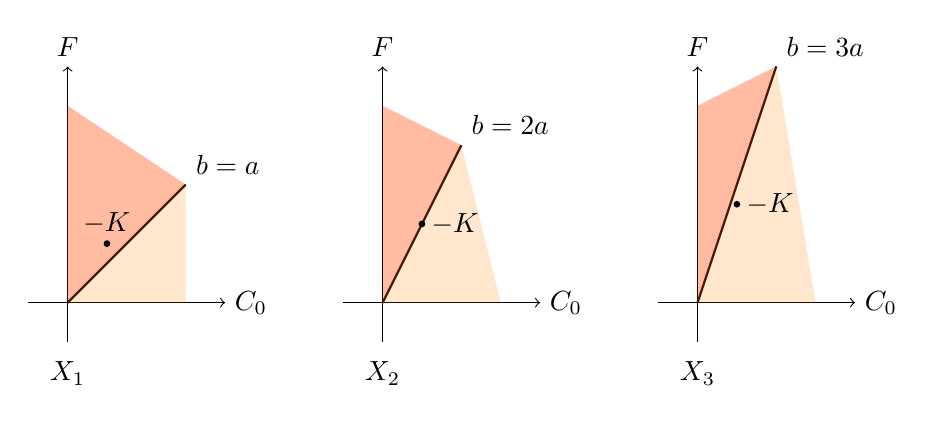
\begin{tikzpicture}[scale=1]
            % First coordinate system
            \begin{scope}[shift={(0,0)}]
                \draw[->] (-0.5,0) -- (2,0) node[right] {$C_0$};
                \draw[->] (0,-0.5) -- (0,3) node[above] {$F$};
                \draw[thick] (0,0) -- (1.5,1.5) node[above right] {$b = a$};
                \fill[red, opacity=0.2] (0,0) -- (1.5,1.5) -- (0,2.5) -- cycle;
                \fill[orange, opacity=0.2] (0,0) -- (0,2.5) -- (1.5,1.5) -- (1.5,0) -- cycle;
                \filldraw[black] (0.5,0.75) circle (1pt);
                \node[above] at (0.5,0.75) {$-K$};
                \node at (0,-0.9) {$X_1$};
            \end{scope}
            % Second coordinate system
            \begin{scope}[shift={(4,0)}]
                \draw[->] (-0.5,0) -- (2,0) node[right] {$C_0$};
                \draw[->] (0,-0.5) -- (0,3) node[above] {$F$};
                \draw[thick] (0,0) -- (1,2) node[above right] {$b = 2a$};
                \fill[red, opacity=0.2] (0,0) -- (1,2) -- (0,2.5) -- cycle;
                \fill[orange, opacity=0.2] (0,0) -- (0,2.5) -- (1,2) -- (1.5,0) -- cycle;
                \filldraw[black] (0.5,1) circle (1pt);
                \node[right] at (0.5,1) {$-K$};
                \node at (0,-0.9) {$X_2$};
            \end{scope}
            % Third coordinate system
            \begin{scope}[shift={(8,0)}]
                \draw[->] (-0.5,0) -- (2,0) node[right] {$C_0$};
                \draw[->] (0,-0.5) -- (0,3) node[above] {$F$};
                \draw[thick] (0,0) -- (1,3) node[above right] {$b = 3a$};
                \fill[red, opacity=0.2] (0,0) -- (1,3) -- (0,2.5) -- cycle;
                \fill[orange, opacity=0.2] (0,0) -- (0,2.5) -- (1,3) -- (1.5,0) -- cycle;
                \filldraw[black] (0.5,1.25) circle (1pt);
                \node[right] at (0.5,1.25) {$-K$};
                \node at (0,-0.9) {$X_3$};
            \end{scope}
        \end{tikzpicture}
        \end{center}
        We have \(-K_{X_e} \equiv 2C_0 + (2+e)F\).
        For \(e=1\), \(-K\) is ample and hence \(X_1\) is a del Pezzo surface.
        For \(e=2\), \(-K\) is nef and big but not ample.
        For \(e\geq 3\), \(-K\) is big but not nef.
    \end{example}


    \paragraph{Elliptic case.} Let \(\pi:X = \bbP_C(\calE) \to E\) be a ruled surface over an elliptic curve \(E\) with \(\calE\) a normalized vector bundle of rank \(2\) and degree \(-e\).

    \begin{theorem}\label{thm:positivity_of_divisors_on_decomposable_ruled_surface_over_elliptic_curve}
        Let \(\pi:X \to E\) be a ruled surface over an elliptic curve \(E\) with invariant \(e\).
        Assume that \(\calE\) is decomposable.
        Let \(C_0\) be a minimal section of \(\pi\) and let \(F\) be a fiber of \(\pi\). 
        Let \(D \equiv aC_0 + bF\) be a divisor on \(X\) with \(a,b \in \bbZ\).
        \begin{enumerate}
            \item \(D\) is effective \(\iff\) \(a \geq 0\) and \(b \geq ae\);
            \item \(D\) is ample \(\iff\) \(D\) is very ample \(\iff\) \(a > 0\) and \(b > ae\).
        \end{enumerate}
    \end{theorem}
    \begin{proof}
        \Yang{To be continued...}
    \end{proof}

    \begin{example}\label{eg:Neron_Severi_group_of_decomposable_ruled_surface_over_elliptic_curve}
        Here we draw the N\'eron-Severi group of the ruled surface \(X\) over an elliptic curve \(E\) with decomposable normalized \(\calE\) for \(e = 1,2,3\).
        \begin{center}
        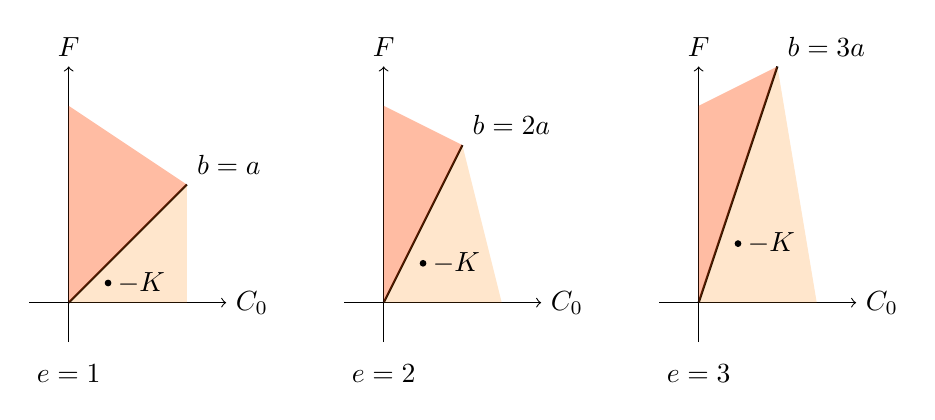
\begin{tikzpicture}[scale=1]
            % First coordinate system
            \begin{scope}[shift={(0,0)}]
                \draw[->] (-0.5,0) -- (2,0) node[right] {$C_0$};
                \draw[->] (0,-0.5) -- (0,3) node[above] {$F$};
                \draw[thick] (0,0) -- (1.5,1.5) node[above right] {$b = a$};
                \fill[red, opacity=0.2] (0,0) -- (1.5,1.5) -- (0,2.5) -- cycle;
                \fill[orange, opacity=0.2] (0,0) -- (0,2.5) -- (1.5,1.5) -- (1.5,0) -- cycle;
                \filldraw[black] (0.5,0.25) circle (1pt);
                \node[right] at (0.5,0.25) {$-K$};
                \node at (0,-0.9) {$e = 1$};
            \end{scope}
            % Second coordinate system
            \begin{scope}[shift={(4,0)}]
                \draw[->] (-0.5,0) -- (2,0) node[right] {$C_0$};
                \draw[->] (0,-0.5) -- (0,3) node[above] {$F$};
                \draw[thick] (0,0) -- (1,2) node[above right] {$b = 2a$};
                \fill[red, opacity=0.2] (0,0) -- (1,2) -- (0,2.5) -- cycle;
                \fill[orange, opacity=0.2] (0,0) -- (0,2.5) -- (1,2) -- (1.5,0) -- cycle;
                \filldraw[black] (0.5,0.5) circle (1pt);
                \node[right] at (0.5,0.5) {$-K$};
                \node at (0,-0.9) {$e = 2$};
            \end{scope}
            % Third coordinate system
            \begin{scope}[shift={(8,0)}]
                \draw[->] (-0.5,0) -- (2,0) node[right] {$C_0$};
                \draw[->] (0,-0.5) -- (0,3) node[above] {$F$};
                \draw[thick] (0,0) -- (1,3) node[above right] {$b = 3a$};
                \fill[red, opacity=0.2] (0,0) -- (1,3) -- (0,2.5) -- cycle;
                \fill[orange, opacity=0.2] (0,0) -- (0,2.5) -- (1,3) -- (1.5,0) -- cycle;
                \filldraw[black] (0.5,0.75) circle (1pt);
                \node[right] at (0.5,0.75) {$-K$};
                \node at (0,-0.9) {$e = 3$};
            \end{scope}
        \end{tikzpicture}
        \end{center}
        In this case, \(-K\equiv 2C_0 + eF\) is always big but not nef.
    \end{example}

    \begin{theorem}\label{thm:positivity_of_divisors_on_indecomposable_ruled_surface_over_elliptic_curve}
        Let \(\pi:X \to E\) be a ruled surface over an elliptic curve \(E\) with invariant \(e\).
        Assume that \(\calE\) is indecomposable.
        Let \(C_0\) be a minimal section of \(\pi\) and let \(F\) be a fiber of \(\pi\). 
        Let \(D \equiv aC_0 + bF\) be a divisor on \(X\) with \(a,b \in \bbZ\).
        \begin{enumerate}
            \item \(D\) is effective \(\iff\) \(a \geq 0\) and \(b \geq \frac{1}{2}ae\);
            \item \(D\) is ample \(\iff\) \(D\) is very ample \(\iff\) \(a > 0\) and \(b > \frac{1}{2}ae\).
        \end{enumerate}
    \end{theorem}
    \begin{proof}
        \Yang{To be continued...}
    \end{proof}

    \begin{example}\label{eg:Neron_Severi_group_of_indecomposable_ruled_surface_over_elliptic_curve}
        Here we draw the N\'eron-Severi group of the ruled surface \(X\) over an elliptic curve \(E\) with indecomposable normalized \(\calE\) for \(e = -1,0\).
        \begin{center}
        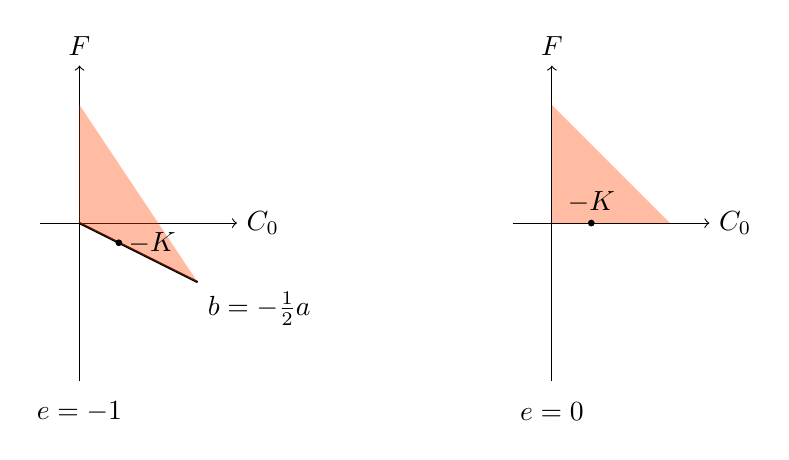
\begin{tikzpicture}[scale=1]
            % First coordinate system
            \begin{scope}[shift={(0,0)}]
                \draw[->] (-0.5,0) -- (2,0) node[right] {$C_0$};
                \draw[->] (0,-2) -- (0,2) node[above] {$F$};
                \draw[thick] (0,0) -- (1.5,-0.75) node[below right] {$b = -\frac{1}{2}a$};
                \fill[red, opacity=0.2] (0,0) -- (1.5,-0.75) -- (0,1.5) -- cycle;
                \fill[orange, opacity=0.2] (0,0) -- (0,1.5) -- (1.5,-0.75) -- cycle;
                \filldraw[black] (0.5,-0.25) circle (1pt);
                \node[right] at (0.5,-0.25) {$-K$};
                \node at (0,-2.4) {$e = -1$};
            \end{scope}
            % Second coordinate system
            \begin{scope}[shift={(6,0)}]
                \draw[->] (-0.5,0) -- (2,0) node[right] {$C_0$};
                \draw[->] (0,-2) -- (0,2) node[above] {$F$};
                % \draw[thick] (0,0) -- (1,1.5) node[above right] {$b = 0$};
                \fill[red, opacity=0.2] (0,0) -- (1.5,0) -- (0,1.5) -- cycle;
                \fill[orange, opacity=0.2] (0,0) -- (1.5,0) -- (0,1.5) -- cycle;
                \filldraw[black] (0.5,0) circle (1pt);
                \node[above] at (0.5,0) {$-K$};
                \node at (0,-2.4) {$e = 0$};
            \end{scope}
        \end{tikzpicture}
        \end{center}
        In this case, \(-K\equiv 2C_0 + eF\) is always nef but not big.
    \end{example}


    \begin{proposition}\label{prop:nef_is_bpf_on_ruled_surface}
        Let \(\pi:X \to C\) be a ruled surface over a smooth curve \(C\).
        Then every nef divisor on \(X\) is semi-ample.
        \Yang{Check this carefully.}
    \end{proposition}

